%% State Space Modelling of Dynamic Systems
%% Lecture 22: Combined Observer and Control
\def\FileDate{10/04/02}
\def\FileVersion{1.0}
% ----------------------------------------------------------------
% Notes pages *********************************************************
% ----------------------------------------------------------------


\begin{center}
	\resizebox{200pt}{!}{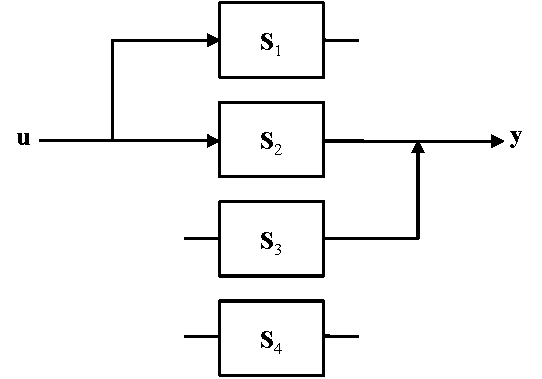
\includegraphics{pictures/partitioning.pdf}}
\end{center}
\endinput

%%% Local Variables: 
%%% mode: latex
%%% TeX-master: "notes"
%%% End:
\ifslidesonly
\begin{slide}
	\heading{Combined Observer and Control}
   
\begin{center}
	\resizebox{200pt}{!}{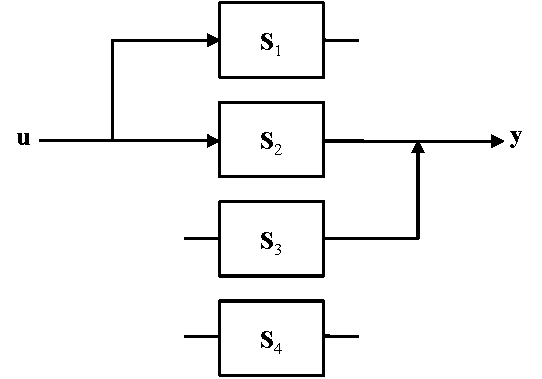
\includegraphics{pictures/partitioning.pdf}}
\end{center}
\endinput

%%% Local Variables: 
%%% mode: latex
%%% TeX-master: "notes"
%%% End:
\end{slide}
\fi

\ifslidesonly
\begin{slide}
	\heading{Contents of this Lecture}
   \begin{itemize}
   	\item Dynamics of the combined controller-observer system
\begin{itemize}
	\item Separation principle
	\item Equivalent classical controller
\end{itemize}
\item Introducing the reference input
\begin{enumerate}
	\item The normal position
	\item Observer driven by the tracking error
\end{enumerate}
   \end{itemize}
\end{slide}
\fi

\section*{Dynamics of the combined system} % (fold)
\label{sub:dynamics_of_the_combined_system}

The vector $[v_{31}, i_{1}]^T$ is called the ``\emph{state
vector}.'' Its elements are state variables.
\endinput
%%% Local Variables: 
%%% mode: latex
%%% TeX-master: "notes"
%%% End: 

\ifslidesonly
\begin{slide}
	\heading{Dynamics of the combined system (1)}
   The vector $[v_{31}, i_{1}]^T$ is called the ``\emph{state
vector}.'' Its elements are state variables.
\endinput
%%% Local Variables: 
%%% mode: latex
%%% TeX-master: "notes"
%%% End: 

\end{slide}
\fi

From previous work the error dynamics are:
\[
\dot{\mathbf{e}} = (\mathbf{A}-\mathbf{LC})\mathbf{e}
\]
Therefore the dynamics of the combined system is:
\[\left[ {\begin{array}{*{20}c}
   {\dot{\mathbf{x}}}  \\
   {\dot{\mathbf{e}}ß}  \\
\end{array}} \right] = \left[ {\begin{array}{*{20}c}
   {\left( {{\bf{A}} - {\bf{BK}}} \right)} & {{\bf{BK}}}  \\
   {\bf{0}} & {\left( {{\bf{A}} - {\bf{LC}}} \right)}  \\
\end{array}} \right]\left[ {\begin{array}{*{20}c}
   {\bf{x}}  \\
   {\bf{e}}  \\
\end{array}} \right] + \left[ {\begin{array}{*{20}c}
   {\bf{B}}  \\
   {\bf{0}}  \\
\end{array}} \right]r
\]
\endinput

%%% Local Variables: 
%%% mode: latex
%%% TeX-master: "notes"
%%% End:
\ifslidesonly
\begin{slide}
	\heading{Dynamics of the combined system (2)}
   From previous work the error dynamics are:
\[
\dot{\mathbf{e}} = (\mathbf{A}-\mathbf{LC})\mathbf{e}
\]
Therefore the dynamics of the combined system is:
\[\left[ {\begin{array}{*{20}c}
   {\dot{\mathbf{x}}}  \\
   {\dot{\mathbf{e}}ß}  \\
\end{array}} \right] = \left[ {\begin{array}{*{20}c}
   {\left( {{\bf{A}} - {\bf{BK}}} \right)} & {{\bf{BK}}}  \\
   {\bf{0}} & {\left( {{\bf{A}} - {\bf{LC}}} \right)}  \\
\end{array}} \right]\left[ {\begin{array}{*{20}c}
   {\bf{x}}  \\
   {\bf{e}}  \\
\end{array}} \right] + \left[ {\begin{array}{*{20}c}
   {\bf{B}}  \\
   {\bf{0}}  \\
\end{array}} \right]r
\]
\endinput

%%% Local Variables: 
%%% mode: latex
%%% TeX-master: "notes"
%%% End:
\end{slide}
\fi 




When the initial conditions of the state-variables are all zero,
this reduces to the transfer matrix model
\begin{equation}\label{eqn:transfer-function}
  \mathbf{Y}=\left[\mathbf{C}\left[s\mathbf{I}-\mathbf{A}\right]^{-1}\mathbf{B}+\mathbf{D}\right]\mathbf{U}
\end{equation}

\endinput

%%% Local Variables: 
%%% mode: latex
%%% TeX-master: "notes"
%%% End: 

\ifslidesonly
\begin{slide}
	\heading{Characteristic Equation (1)}
   When the initial conditions of the state-variables are all zero,
this reduces to the transfer matrix model
\begin{equation}\label{eqn:transfer-function}
  \mathbf{Y}=\left[\mathbf{C}\left[s\mathbf{I}-\mathbf{A}\right]^{-1}\mathbf{B}+\mathbf{D}\right]\mathbf{U}
\end{equation}

\endinput

%%% Local Variables: 
%%% mode: latex
%%% TeX-master: "notes"
%%% End: 

\end{slide}
\fi

When the observer canonical form is not used, then the design of the observer is more difficult. Ackermann's formula can be adapted as follows:
% MathType!MTEF!2!1!+-
% faaagaart1ev2aaaKnaaaaWenf2ys9wBH5garuavP1wzZbqedmvETj
% 2BSbqefm0B1jxALjharqqtubsr4rNCHbGeaGqiVu0Je9sqqrpepC0x
% bbL8FesqqrFfpeea0xe9Lq-Jc9vqaqpepm0xbba9pwe9Q8fs0-yqaq
% pepae9pg0FirpepeKkFr0xfr-xfr-xb9Gqpi0dc9adbaqaaeGaciGa
% aiaabeqaamaabaabaaGcbaGaaCitamaaCaaaleqabaGaamivaaaaki
% abg2da9maadmaabaqbamqabeabaaaabaGaaGimaaqaaiablAcilbqa
% aiaaicdaaeaacaaIXaaaaaGaay5waiaaw2faaiaad+eadaahaaWcbe
% qaaiabgkHiTiaaigdaaaGccqaHXoqydaWgaaWcbaGaam4yaaqabaGc
% caGGOaGaaCyqamaaCaaaleqabaGaamivaaaakiaacMcaaaa!3EF6!
\[
{\bf{L}}^T  = \left[ {\begin{array}{*{20}c}
   0 &  \ldots  & 0 & 1  \\
\end{array}} \right]\mathcal{O}^{ - 1} \alpha _e ({\bf{A}}^T )
\]
$\mathcal{O}$ is the observability matrix:
\[
\mathcal{O}=[\mathbf{C}^T\vdots\mathbf{A}^T\mathbf{C}^T\vdots\cdots\vdots(\mathbf{A}^T)^{n-1}\mathbf{C}^T]
\]
and if $\alpha_e(s)=s^n + \alpha_1s^{n-1}+\cdots+\alpha_n$ then \[\alpha_e(\mathbf{A}^T)=(\mathbf{A}^T)^n + \alpha_1(\mathbf{A}^T)^{n-1}+\cdots+\mathbf{I}\alpha_n.\]
 

Notice that if the system is unobservable, then the matrix inverse $\mathcal{O}^{-1}$ does not exist and we cannot design an observer for this system.


 
 

\endinput

%%% Local Variables: 
%%% mode: latex
%%% TeX-master: "notes"
%%% End:
\ifslidesonly
\begin{slide}
	\heading{Characteristic Equation (2)}
   When the observer canonical form is not used, then the design of the observer is more difficult. Ackermann's formula can be adapted as follows:
% MathType!MTEF!2!1!+-
% faaagaart1ev2aaaKnaaaaWenf2ys9wBH5garuavP1wzZbqedmvETj
% 2BSbqefm0B1jxALjharqqtubsr4rNCHbGeaGqiVu0Je9sqqrpepC0x
% bbL8FesqqrFfpeea0xe9Lq-Jc9vqaqpepm0xbba9pwe9Q8fs0-yqaq
% pepae9pg0FirpepeKkFr0xfr-xfr-xb9Gqpi0dc9adbaqaaeGaciGa
% aiaabeqaamaabaabaaGcbaGaaCitamaaCaaaleqabaGaamivaaaaki
% abg2da9maadmaabaqbamqabeabaaaabaGaaGimaaqaaiablAcilbqa
% aiaaicdaaeaacaaIXaaaaaGaay5waiaaw2faaiaad+eadaahaaWcbe
% qaaiabgkHiTiaaigdaaaGccqaHXoqydaWgaaWcbaGaam4yaaqabaGc
% caGGOaGaaCyqamaaCaaaleqabaGaamivaaaakiaacMcaaaa!3EF6!
\[
{\bf{L}}^T  = \left[ {\begin{array}{*{20}c}
   0 &  \ldots  & 0 & 1  \\
\end{array}} \right]\mathcal{O}^{ - 1} \alpha _e ({\bf{A}}^T )
\]
$\mathcal{O}$ is the observability matrix:
\[
\mathcal{O}=[\mathbf{C}^T\vdots\mathbf{A}^T\mathbf{C}^T\vdots\cdots\vdots(\mathbf{A}^T)^{n-1}\mathbf{C}^T]
\]
and if $\alpha_e(s)=s^n + \alpha_1s^{n-1}+\cdots+\alpha_n$ then \[\alpha_e(\mathbf{A}^T)=(\mathbf{A}^T)^n + \alpha_1(\mathbf{A}^T)^{n-1}+\cdots+\mathbf{I}\alpha_n.\]
 

Notice that if the system is unobservable, then the matrix inverse $\mathcal{O}^{-1}$ does not exist and we cannot design an observer for this system.


 
 

\endinput

%%% Local Variables: 
%%% mode: latex
%%% TeX-master: "notes"
%%% End:
\end{slide}
\fi


% section dynamics_of_the_combined_system (end)




\subsection*{Separation Principle} % (fold)
\label{sub:separation_principle}

From the above work, we can conclude that the set of poles of the combined observer-controller system is the union of the set of closed loop controller poles and the set of observer poles.

The controller matrix  $\mathbf{K}$  is designed as before, as if the real plant states are going to be used for the feedback. This fixes the positions of the controller poles into the desired positions.

Then, quite independently, the matrix $\mathbf{L}$ is designed as before to fix the observer poles as required.

Using the observer states for the control feedback instead of the plant states does not affect the closed loop poles.

This is a fortunate situation and is known as the \textbf{separation principle}. The problems of controller design and observer design have been separated.

\ifslidesonly
\begin{slide}
	\heading{Separation Principle}
	\begin{itemize}
		\item Poles of the combined observer-controller system is the union of closed loop controller and observer poles.
		\item The controller matrix  $\mathbf{K}$  is designed as before.
		\item Quite independently, the matrix $\mathbf{L}$ is designed to fix the observer poles as required.
		\item Using the observer states for the control feedback instead of the plant states does not affect the closed loop poles.
	\end{itemize}
   This is a fortunate situation and is known as the \textbf{separation principle}. The problems of controller design and observer design have been separated.
\end{slide}
\fi
 
% section separation_principle (end)


\subsection*{The Equivalent Classical Compensator} % (fold)
\label{sec:the_equivalent_classical_compensator}


The matrix function becomes:
\begin{eqnarray*}
	f(\mathbf{A}t) & = & f_0\mathbf{TIT}^{-1} + f_1\mathbf{T\Lambda T}^{-1}t + f_2\mathbf{T\Lambda}^2\mathbf{T}^{-1}t^2 + \cdots + f_n\mathbf{T\Lambda}^n\mathbf{T}^{-1}t^n + \cdots \\
	f(\mathbf{A}t) & = & \mathbf{T}\left(f_0\mathbf{I} + f_1\mathbf{\Lambda}t + f_2\mathbf{\Lambda}^2t^2 + \cdots + f_n\mathbf{\Lambda}^nt^n + \cdots \right)\mathbf{T}^{-1}\\
	               & = & \mathbf{T}f(\mathbf{\Lambda}t)\mathbf{T}^{-1}
\end{eqnarray*}
 
The term inside the brackets on the rhs is a diagonal matrix and the $i^\mathrm{th}$ diagonal element is:
\[
f_0+f_1\lambda_it + f_2\lambda_i^2t^2 + \cdots + f_n\lambda_i^nt^ + \cdots
\]
From the Taylor series this must be $f(\lambda_i t)$:
\[
f(\mathbf{A} t)=\mathbf{T} f(\mathbf{\Lambda} t) \mathbf{T}^{-1}
\]   
where $f(\mathbf{\Lambda} t)=\mathrm{diag}\left(f(\lambda_i t)\right)$.

\endinput

%%% Local Variables: 
%%% mode: latex
%%% TeX-master: "notes"
%%% End:
\ifslidesonly
\begin{slide}
	\heading{The Equivalent Classical Compensator}
	The matrix function becomes:
\begin{eqnarray*}
	f(\mathbf{A}t) & = & f_0\mathbf{TIT}^{-1} + f_1\mathbf{T\Lambda T}^{-1}t + f_2\mathbf{T\Lambda}^2\mathbf{T}^{-1}t^2 + \cdots + f_n\mathbf{T\Lambda}^n\mathbf{T}^{-1}t^n + \cdots \\
	f(\mathbf{A}t) & = & \mathbf{T}\left(f_0\mathbf{I} + f_1\mathbf{\Lambda}t + f_2\mathbf{\Lambda}^2t^2 + \cdots + f_n\mathbf{\Lambda}^nt^n + \cdots \right)\mathbf{T}^{-1}\\
	               & = & \mathbf{T}f(\mathbf{\Lambda}t)\mathbf{T}^{-1}
\end{eqnarray*}
 
The term inside the brackets on the rhs is a diagonal matrix and the $i^\mathrm{th}$ diagonal element is:
\[
f_0+f_1\lambda_it + f_2\lambda_i^2t^2 + \cdots + f_n\lambda_i^nt^ + \cdots
\]
From the Taylor series this must be $f(\lambda_i t)$:
\[
f(\mathbf{A} t)=\mathbf{T} f(\mathbf{\Lambda} t) \mathbf{T}^{-1}
\]   
where $f(\mathbf{\Lambda} t)=\mathrm{diag}\left(f(\lambda_i t)\right)$.

\endinput

%%% Local Variables: 
%%% mode: latex
%%% TeX-master: "notes"
%%% End:
\end{slide}
\fi


Setting the reference input $r = 0$  gives:
\begin{itemize}
	\item Rule of thumb: observer poles can be faster than the controller poles (i.e. further from the origin) by a factor of 2 to 6. This makes the effect of the observer dynamics short-term and the overall response is dominated by the controller poles.
	\item If noise/disturbance is present this has an effect on the choice:
	\begin{description}
		\item[Process noise $w$:] $d\mathbf{x}/dt=\mathbf{Ax}+\mathbf{B}u+\mathbf{B}_1 w$
		\item[Sensor noise $v$:]  $y = \mathbf{C}x+v$
		\item[Observer:] $d\hat{\mathbf{x}}=\mathbf{A}\hat{\mathbf{x}}+\mathbf{B}u+\mathbf{L}(y-\mathbf{C}\hat{\mathbf{x}})$
		\item[Error $\mathbf{e}=\mathbf{x}-\hat{\mathbf{x}}$:] $d\mathbf{e}/dt=(\mathbf{A}-\mathbf{LC})\mathbf{e}+\mathbf{B}_1 w - \mathbf{L}v.$
	\end{description}
\end{itemize}

\endinput

%%% Local Variables: 
%%% mode: latex
%%% TeX-master: "notes"
%%% End:
\ifslidesonly
\begin{slide}
	\heading{When $r=0$}
   \begin{itemize}
	\item Rule of thumb: observer poles can be faster than the controller poles (i.e. further from the origin) by a factor of 2 to 6. This makes the effect of the observer dynamics short-term and the overall response is dominated by the controller poles.
	\item If noise/disturbance is present this has an effect on the choice:
	\begin{description}
		\item[Process noise $w$:] $d\mathbf{x}/dt=\mathbf{Ax}+\mathbf{B}u+\mathbf{B}_1 w$
		\item[Sensor noise $v$:]  $y = \mathbf{C}x+v$
		\item[Observer:] $d\hat{\mathbf{x}}=\mathbf{A}\hat{\mathbf{x}}+\mathbf{B}u+\mathbf{L}(y-\mathbf{C}\hat{\mathbf{x}})$
		\item[Error $\mathbf{e}=\mathbf{x}-\hat{\mathbf{x}}$:] $d\mathbf{e}/dt=(\mathbf{A}-\mathbf{LC})\mathbf{e}+\mathbf{B}_1 w - \mathbf{L}v.$
	\end{description}
\end{itemize}

\endinput

%%% Local Variables: 
%%% mode: latex
%%% TeX-master: "notes"
%%% End:
\end{slide}
\fi

Taking Laplace transforms, ignoring ICs:
The last example had a system TF with no zeros. In this case it is easy to construct the equivalent classical controller. We had the feedback law:
\[
u=r-5x_1-156x_2
\]

Now $y=7x_2$ and $\dot{x}_2=x_1$ therefore $X_2(s)=Y(s)/7$ and $X_1(s)=sX_2(s)=sY(s)/7$. Therefore
\begin{eqnarray*}
	U(s) & = & R(s)-rX_1(s)-156X_2(s) \\
	& = & R(s) - \frac{1}{7}(5s+156)Y(s)
\end{eqnarray*}

\endinput

%%% Local Variables: 
%%% mode: latex
%%% TeX-master: "notes"
%%% End:
\ifslidesonly
\begin{slide}
	\heading{Taking Laplace Transforms}
   The last example had a system TF with no zeros. In this case it is easy to construct the equivalent classical controller. We had the feedback law:
\[
u=r-5x_1-156x_2
\]

Now $y=7x_2$ and $\dot{x}_2=x_1$ therefore $X_2(s)=Y(s)/7$ and $X_1(s)=sX_2(s)=sY(s)/7$. Therefore
\begin{eqnarray*}
	U(s) & = & R(s)-rX_1(s)-156X_2(s) \\
	& = & R(s) - \frac{1}{7}(5s+156)Y(s)
\end{eqnarray*}

\endinput

%%% Local Variables: 
%%% mode: latex
%%% TeX-master: "notes"
%%% End:
\end{slide}
\fi


Alternatively, since
\[
s{\bf{\hat X}}(s) =  {\bf{A\hat X}}(s) + {\bf{B}}U(s) + {\bf{L}}\left( {Y(s) - {\bf{C\hat X}}}(s) \right)
\]
then,
\[
\left( {s{\bf{I}} - {\bf{A}} + {\bf{LC}}} \right){\bf{\hat X}}(s) = {\bf{B}}U(s) + {\bf{L}}Y(s) 
\]
or,
\[
{\bf{\hat X}}(s) = {\bf{M}}^{ - 1} {\bf{B}}U(s) + {\bf{M}}^{ - 1} {\bf{L}}Y(s)
\]


\endinput

%%% Local Variables: 
%%% mode: latex
%%% TeX-master: "notes"
%%% End:
\ifslidesonly
\begin{slide}
	\heading{Alternative Formulation (1)}
   \[
s{\bf{\hat X}}(s) =  {\bf{A\hat X}}(s) + {\bf{B}}U(s) + {\bf{L}}\left( {Y(s) - {\bf{C\hat X}}}(s) \right)
\]
then,
\[
\left( {s{\bf{I}} - {\bf{A}} + {\bf{LC}}} \right){\bf{\hat X}}(s) = {\bf{B}}U(s) + {\bf{L}}Y(s) 
\]
or,
\[
{\bf{\hat X}}(s) = {\bf{M}}^{ - 1} {\bf{B}}U(s) + {\bf{M}}^{ - 1} {\bf{L}}Y(s)
\]


\endinput

%%% Local Variables: 
%%% mode: latex
%%% TeX-master: "notes"
%%% End:
\end{slide}
\fi
Now
\[
U(s) =  - {\bf{K\hat X}}(s) 
\]
so
\[
U (s) =   - {\bf{K}}\left( {{\bf{M}}^{ - 1} {\bf{B}}U(s) + {\bf{M}}^{ - 1} {\bf{L}}Y(s)} \right) 
\]
\[
 \left( {1 + {\bf{KM}}^{ - 1} {\bf{B}}} \right)U(s) =  - {\bf{KM}}^{ - 1} {\bf{L}}Y(s)
\]

\[ 
H\left( s \right) =  - \frac{U(s)}{Y(sßß)} = \frac{{{\bf{KM}}^{ - 1} {\bf{L}}}}{{1 + {\bf{KM}}^{ - 1} {\bf{B}}}} 
\]




\endinput

%%% Local Variables: 
%%% mode: latex
%%% TeX-master: "notes"
%%% End:
\ifslidesonly
\begin{slide}
	\heading{Alternative Formulation (2)}
   Now
\[
U(s) =  - {\bf{K\hat X}}(s) 
\]
so
\[
U (s) =   - {\bf{K}}\left( {{\bf{M}}^{ - 1} {\bf{B}}U(s) + {\bf{M}}^{ - 1} {\bf{L}}Y(s)} \right) 
\]
\[
 \left( {1 + {\bf{KM}}^{ - 1} {\bf{B}}} \right)U(s) =  - {\bf{KM}}^{ - 1} {\bf{L}}Y(s)
\]

\[ 
H\left( s \right) =  - \frac{U(s)}{Y(sßß)} = \frac{{{\bf{KM}}^{ - 1} {\bf{L}}}}{{1 + {\bf{KM}}^{ - 1} {\bf{B}}}} 
\]




\endinput

%%% Local Variables: 
%%% mode: latex
%%% TeX-master: "notes"
%%% End:
\end{slide}
\fi

% section the_equivalent_classical_compensator (end)



 
\section*{Introducing the Reference Input} % (fold)
\label{sec:introducing_the_reference_input}

\ifslidesonly
\begin{slide}
   \heading{Introducing the Reference Input}
Two cases considered:
\begin{enumerate}
	\item The Normal Position
	\begin{itemize}
		\item The reference input is introduced as $u=r-\mathbf{K}\hat{\mathbf{x}}$.
	\end{itemize}
	\item Observer driven by the tracking error
	\begin{itemize}
		\item Sense the tracking error and use this to control the system.
		\item The tracking error is the difference between the desired and actual outputs $\tilde e =  - r + y$
	\end{itemize}
	Systems in each case have different properties.
\end{enumerate}
   
\end{slide}
\fi
\subsection*{1. The Normal Position} % (fold)
\label{sub:1_the_normal_position}

Given the transformation $\mathbf{T}^{-1}\mathbf{AT}=\mathbf{\Lambda}$:
\begin{eqnarray*}
	\mathbf{A}t & = & (\mathbf{T\Lambda T}^{-1}) t \\
	\mathbf{A}^nt^n & = & (\mathbf{T\Lambda T}^{-1})(\mathbf{T\Lambda T}^{-1})\ldots(\mathbf{T\Lambda T}^{-1})t^n \\
	                & = & \mathbf{T\Lambda T}^{-1}\mathbf{T\Lambda T}^{-1}\ldots\mathbf{T\Lambda T}^{-1}t^n \\
	\mathbf{A}^nt^n & = & \mathbf{T\Lambda}\mathbf{I}\mathbf{\Lambda I}\ldots\mathbf{I\Lambda T}^{-1}t^n \\
	\               & = & \mathbf{T\Lambda}^n\mathbf{T}^{-1}t^n \\
\end{eqnarray*}
\endinput

%%% Local Variables: 
%%% mode: latex
%%% TeX-master: "notes"
%%% End:
\ifslidesonly
\begin{slide}
	\heading{1. The Normal Position}
   Given the transformation $\mathbf{T}^{-1}\mathbf{AT}=\mathbf{\Lambda}$:
\begin{eqnarray*}
	\mathbf{A}t & = & (\mathbf{T\Lambda T}^{-1}) t \\
	\mathbf{A}^nt^n & = & (\mathbf{T\Lambda T}^{-1})(\mathbf{T\Lambda T}^{-1})\ldots(\mathbf{T\Lambda T}^{-1})t^n \\
	                & = & \mathbf{T\Lambda T}^{-1}\mathbf{T\Lambda T}^{-1}\ldots\mathbf{T\Lambda T}^{-1}t^n \\
	\mathbf{A}^nt^n & = & \mathbf{T\Lambda}\mathbf{I}\mathbf{\Lambda I}\ldots\mathbf{I\Lambda T}^{-1}t^n \\
	\               & = & \mathbf{T\Lambda}^n\mathbf{T}^{-1}t^n \\
\end{eqnarray*}
\endinput

%%% Local Variables: 
%%% mode: latex
%%% TeX-master: "notes"
%%% End:
\end{slide}
\fi



\subsubsection*{Finding $F(s)$ and $H(s)$} % (fold)
\label{ssub:finding_f_s_and_h_s_}

For the observer we have:
$\mathcal{C}$ is the controllability matrix (see Lecture 19):
\[
\mathcal{C} = [\mathbf{B}\vdots\mathbf{AB}\vdots\cdots\vdots\mathbf{A}^{n-1}\mathbf{B}]
\]
and
\[
\alpha_c(\mathbf{A})=\mathbf{A}^n + \alpha_1\mathbf{A}^{n-1}+ \cdots + \alpha_n\mathbf{I}
\]

\endinput

%%% Local Variables: 
%%% mode: latex
%%% TeX-master: "notes"
%%% End:
\ifslidesonly
\begin{slide}
	\heading{Finding$F(s)$ and $H(s)$: Observer}
   $\mathcal{C}$ is the controllability matrix (see Lecture 19):
\[
\mathcal{C} = [\mathbf{B}\vdots\mathbf{AB}\vdots\cdots\vdots\mathbf{A}^{n-1}\mathbf{B}]
\]
and
\[
\alpha_c(\mathbf{A})=\mathbf{A}^n + \alpha_1\mathbf{A}^{n-1}+ \cdots + \alpha_n\mathbf{I}
\]

\endinput

%%% Local Variables: 
%%% mode: latex
%%% TeX-master: "notes"
%%% End:
\end{slide}
\fi

For the controller we have:
\[
u = r - \mathbf{K}\hat{\mathbf{x}}
\]
Taking Laplace transforms
\[
U = R - \mathbf{K}\hat{\mathbf{X}}
\]

\endinput

%%% Local Variables: 
%%% mode: latex
%%% TeX-master: "notes"
%%% End:
\ifslidesonly
\begin{slide}
	\heading{Finding$F(s)$ and $H(s)$: Controller}
   \[
u = r - \mathbf{K}\hat{\mathbf{x}}
\]
Taking Laplace transforms
\[
U = R - \mathbf{K}\hat{\mathbf{X}}
\]

\endinput

%%% Local Variables: 
%%% mode: latex
%%% TeX-master: "notes"
%%% End:
\end{slide}
\fi

Therefore, for the combined observer-controller
\[
U=R-\mathbf{K}\left(\mathbf{M}^{-1}\mathbf{B}U + \mathbf{M}^{-1}{\bf{L}}Y\right)
\]
Re-arranging:
\[
\left(\mathbf{KM}^{-1}\mathbf{B}+1\right)U=R-\mathbf{KM}^{-1}\mathbf{L}Y
\]
therefore,
\[
U=\frac{1}{\mathbf{KM}^{-1}\mathbf{B}+1}R-\frac{\mathbf{KM}^{-1}\mathbf{L}}{\mathbf{KM}^{-1}\mathbf{B}+1}Y
\]

\endinput

%%% Local Variables: 
%%% mode: latex
%%% TeX-master: "notes"
%%% End:
\ifslidesonly
\begin{slide}
	\heading{Finding$F(s)$ and $H(s)$: Combined Observer-Controller}
   \[
U=R-\mathbf{K}\left(\mathbf{M}^{-1}\mathbf{B}U + \mathbf{M}^{-1}{\bf{L}}Y\right)
\]
Re-arranging:
\[
\left(\mathbf{KM}^{-1}\mathbf{B}+1\right)U=R-\mathbf{KM}^{-1}\mathbf{L}Y
\]
therefore,
\[
U=\frac{1}{\mathbf{KM}^{-1}\mathbf{B}+1}R-\frac{\mathbf{KM}^{-1}\mathbf{L}}{\mathbf{KM}^{-1}\mathbf{B}+1}Y
\]

\endinput

%%% Local Variables: 
%%% mode: latex
%%% TeX-master: "notes"
%%% End:
\end{slide}
\fi


Comparing with: $$U=F(s)R-H(s)Y$$
\[
F(s) = \frac{1}{\mathbf{KM}^{-1}\mathbf{B}+1}
\]
and
\[
H(s) = \frac{\mathbf{KM}^{-1}\mathbf{L}}{\mathbf{KM}^{-1}\mathbf{B}+1}
\]

% subsubsection finding_f_s_and_h_s_ (end)

 

\subsubsection*{A useful theorem} % (fold)
\label{ssub:a_useful_theorem}

Since,
\[
u = r - \mathbf{Kx}
\]
then the closed-loop system is:
\begin{eqnarray*}
	\dot{\mathbf{x}} & = & \mathbf{A}\mathbf{x}+\mathbf{B}u;\ y = \mathbf{C}\mathbf{x}+\mathbf{D}u \\
	\dot{\mathbf{x}} & = & \mathbf{A}\mathbf{x}+\mathbf{B}(r - \mathbf{K}\mathbf{x});\ y = \mathbf{C}\mathbf{x}+\mathbf{D}(r - \mathbf{K}\mathbf{x}) \\
	\dot{\mathbf{x}} & = & (\mathbf{A}-\mathbf{B}\mathbf{K})\mathbf{x}+\mathbf{B}r;\ y = (\mathbf{C}-\mathbf{D}\mathbf{K})\mathbf{x}+\mathbf{D}r \\
\end{eqnarray*}

\endinput

%%% Local Variables: 
%%% mode: latex
%%% TeX-master: "notes"
%%% End:
\ifslidesonly
\begin{slide}
	\heading{A Useful Theorem}
   Since,
\[
u = r - \mathbf{Kx}
\]
then the closed-loop system is:
\begin{eqnarray*}
	\dot{\mathbf{x}} & = & \mathbf{A}\mathbf{x}+\mathbf{B}u;\ y = \mathbf{C}\mathbf{x}+\mathbf{D}u \\
	\dot{\mathbf{x}} & = & \mathbf{A}\mathbf{x}+\mathbf{B}(r - \mathbf{K}\mathbf{x});\ y = \mathbf{C}\mathbf{x}+\mathbf{D}(r - \mathbf{K}\mathbf{x}) \\
	\dot{\mathbf{x}} & = & (\mathbf{A}-\mathbf{B}\mathbf{K})\mathbf{x}+\mathbf{B}r;\ y = (\mathbf{C}-\mathbf{D}\mathbf{K})\mathbf{x}+\mathbf{D}r \\
\end{eqnarray*}

\endinput

%%% Local Variables: 
%%% mode: latex
%%% TeX-master: "notes"
%%% End:
\end{slide}
\fi

 
% subsubsection a_useful_theorem (end)
\subsubsection*{Zeros and Poles of $F(s)$ and $H(s)$} % (fold)
\label{ssub:zeros_and_poles_of_f_s_and_h_s_}

Applying the theorem:
\[
\mathbf{KM}^{-1}\mathbf{B}+1=\frac{\det\left(\mathbf{M}+\mathbf{BK}\right)}{\det{\mathbf{M}}}
\]
therefore,
\[
F(s) = \frac{\det\mathbf{M}}{\det\left(\mathbf{M}+\mathbf{BK}\right)}
\]


\endinput

%%% Local Variables: 
%%% mode: latex
%%% TeX-master: "notes"
%%% End:
\ifslidesonly
\begin{slide}
	\heading{Zeros and Poles of $F(s)$ (1)}
   Applying the theorem:
\[
\mathbf{KM}^{-1}\mathbf{B}+1=\frac{\det\left(\mathbf{M}+\mathbf{BK}\right)}{\det{\mathbf{M}}}
\]
therefore,
\[
F(s) = \frac{\det\mathbf{M}}{\det\left(\mathbf{M}+\mathbf{BK}\right)}
\]


\endinput

%%% Local Variables: 
%%% mode: latex
%%% TeX-master: "notes"
%%% End:
\end{slide}
\fi

Adding $\mathbf{K}$ times the $2^\mathrm{nd}$ column to the first cancels terms whilst leaving the determinant unchanged.

The new form for the TF is:
\[
\frac{{Y(s)}}{{R(s)}} = \frac{{\det \left[ {\begin{array}{*{20}c}
   {(s{\bf{I}} - {\bf{A}})} & { - {\bf{B}}}  \\
   {\bf{C}} & {\bf{D}}  \\
\end{array}} \right]}}{{\det (s{\bf{I}} - {\bf{A}} + {\bf{BK}})}}
\]

Notice now that numerator is identical to that of the open loop TF. This implies that the state feedback control has left the open loop zeros unchanged. The different denominator is due to the feedback action which alters the pole positions as required.

\endinput

%%% Local Variables: 
%%% mode: latex
%%% TeX-master: "notes"
%%% End:
\ifslidesonly
\begin{slide}
	\heading{Zeros and Poles of $F(s)$ (2)}
   Adding $\mathbf{K}$ times the $2^\mathrm{nd}$ column to the first cancels terms whilst leaving the determinant unchanged.

The new form for the TF is:
\[
\frac{{Y(s)}}{{R(s)}} = \frac{{\det \left[ {\begin{array}{*{20}c}
   {(s{\bf{I}} - {\bf{A}})} & { - {\bf{B}}}  \\
   {\bf{C}} & {\bf{D}}  \\
\end{array}} \right]}}{{\det (s{\bf{I}} - {\bf{A}} + {\bf{BK}})}}
\]

Notice now that numerator is identical to that of the open loop TF. This implies that the state feedback control has left the open loop zeros unchanged. The different denominator is due to the feedback action which alters the pole positions as required.

\endinput

%%% Local Variables: 
%%% mode: latex
%%% TeX-master: "notes"
%%% End:
\end{slide}
\fi

Similarly for $H(s)$:
When a zero is close to a pole in the TF there is a marked increase in the feedback gains. This effect is best illustrated with an example.

Given a system with a TF,
\[
\frac{Y(s)}{U(s)}=\frac{s-z}{s-p}=1+\frac{p-z}{s-p}
\]
find the control law to move the pole to $p_c$.



\endinput

%%% Local Variables: 
%%% mode: latex
%%% TeX-master: "notes"
%%% End:
\ifslidesonly
\begin{slide}
	\heading{Zeros and Poles of $H(s)$}
   When a zero is close to a pole in the TF there is a marked increase in the feedback gains. This effect is best illustrated with an example.

Given a system with a TF,
\[
\frac{Y(s)}{U(s)}=\frac{s-z}{s-p}=1+\frac{p-z}{s-p}
\]
find the control law to move the pole to $p_c$.



\endinput

%%% Local Variables: 
%%% mode: latex
%%% TeX-master: "notes"
%%% End:
\end{slide}
\fi


% subsubsection zeros_and_poles_of_f_s_and_h_s_ (end)


\subsubsection*{The Overall Closed Loop TF} % (fold)
\label{ssub:the_overall_closed_loop_tf}

Using the observer canonical form,
\[
\dot{x}=px+(p - z)u,\ y = x + u.
\]

Design the feedback to move the closed-loop pole to $p_c$.
Now,
\[
\mathbf{A}=p;\ \mathbf{B}=p-z;\ \mathbf{K}=k_1.
\]
Desired CE polynomial: $\alpha_c(s)=s-p_c$. Actual CE polynomial: 
$\det(s\mathbf{I}-\mathbf{A}-\mathbf{BK}) = s - p + (p - z)k_1.$

Comparing the constant:
\begin{eqnarray*}
	-p_c & = & -p + (p - z)k_1 \\
	k_1 & = & \frac{p-p_c}{p-z}
\end{eqnarray*}


\endinput

%%% Local Variables: 
%%% mode: latex
%%% TeX-master: "notes"
%%% End:
\ifslidesonly
\begin{slide}
	\heading{The Overall Closed Loop TF (1)}
   Using the observer canonical form,
\[
\dot{x}=px+(p - z)u,\ y = x + u.
\]

Design the feedback to move the closed-loop pole to $p_c$.
Now,
\[
\mathbf{A}=p;\ \mathbf{B}=p-z;\ \mathbf{K}=k_1.
\]
Desired CE polynomial: $\alpha_c(s)=s-p_c$. Actual CE polynomial: 
$\det(s\mathbf{I}-\mathbf{A}-\mathbf{BK}) = s - p + (p - z)k_1.$

Comparing the constant:
\begin{eqnarray*}
	-p_c & = & -p + (p - z)k_1 \\
	k_1 & = & \frac{p-p_c}{p-z}
\end{eqnarray*}


\endinput

%%% Local Variables: 
%%% mode: latex
%%% TeX-master: "notes"
%%% End:
\end{slide}
\fi

Notice that the feedback gain $k_{1}$ is large if:
\begin{itemize}
	\item the zero is close to the pole: $z\approx p$
	\item the closed loop pole $p_c$ is far from $p$
\end{itemize}

\endinput

%%% Local Variables: 
%%% mode: latex
%%% TeX-master: "notes"
%%% End:
\ifslidesonly
\begin{slide}
	\heading{The Overall Closed Loop TF (2)}
   Notice that the feedback gain $k_{1}$ is large if:
\begin{itemize}
	\item the zero is close to the pole: $z\approx p$
	\item the closed loop pole $p_c$ is far from $p$
\end{itemize}

\endinput

%%% Local Variables: 
%%% mode: latex
%%% TeX-master: "notes"
%%% End:
\end{slide}
\fi

\begin{itemize}
	\item Notice here how the input TF $F(s)$ contains as its zeros all the poles of the observer given by $\alpha_e(s)$.
	\item Because of the separation principle, these are also half of the poles of the overall closed loop TF.
	\item The pole-zero cancellation results in the final TF having just the plant zeros and the controller poles.
	\item Thus we can say that, using the observer states for the feedback, instead of the unavailable plant states, has not affected the closed loop TF.
	\item This is not the case when the reference input is introduced elsewhere.
\end{itemize}


\endinput

%%% Local Variables: 
%%% mode: latex
%%% TeX-master: "notes"
%%% End:
\ifslidesonly
\begin{slide}
	\heading{The Overall Closed Loop TF: Comments}
   \begin{itemize}
	\item Notice here how the input TF $F(s)$ contains as its zeros all the poles of the observer given by $\alpha_e(s)$.
	\item Because of the separation principle, these are also half of the poles of the overall closed loop TF.
	\item The pole-zero cancellation results in the final TF having just the plant zeros and the controller poles.
	\item Thus we can say that, using the observer states for the feedback, instead of the unavailable plant states, has not affected the closed loop TF.
	\item This is not the case when the reference input is introduced elsewhere.
\end{itemize}


\endinput

%%% Local Variables: 
%%% mode: latex
%%% TeX-master: "notes"
%%% End:
\end{slide}
\fi



% subsubsection the_overall_closed_loop_tf (end)

% subsection 1_the_normal_position (end)


 
\subsection*{2. Observer Driven by the Tracking Error
} % (fold)
\label{sub:2_observer_driven_by_the_tracking_error_}

Sometimes it is desired to sense the tracking error and use this to control the system.

The tracking error is the difference between the desired and actual outputs,
\[
\tilde e =  - r + y
\]

 
Some sensors can only measure a difference between two measurands. eg  a thermocouple can only sense the temperature difference between its hot and cold junctions.
\begin{center}
	\resizebox{!}{2in}{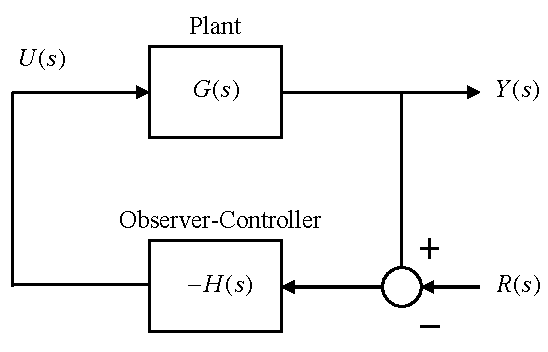
\includegraphics{pictures/fig3.pdf}}
\end{center}
\ifslidesonly
\begin{slide}
   \heading{2. Observer Driven by the Tracking Error}
The tracking error is the difference between the desired and actual outputs,
\[
\tilde e =  - r + y
\]
   \begin{center}
	\resizebox{200pt}{!}{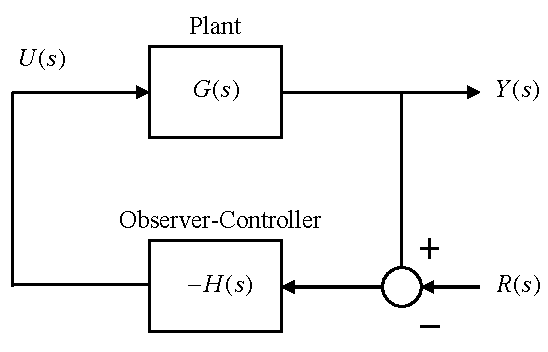
\includegraphics{pictures/fig3.pdf}}
   \end{center}
\end{slide}
\fi
Redraw:
\begin{center}
	\resizebox{250pt}{!}{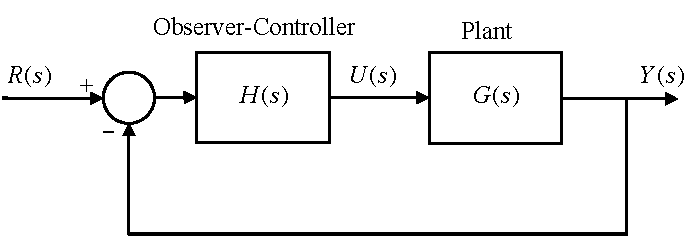
\includegraphics{pictures/fig4.pdf}}
\end{center}
\ifslidesonly
\begin{slide}
   \heading{Redraw Block Diagram}
   \begin{center}
	\resizebox{250pt}{!}{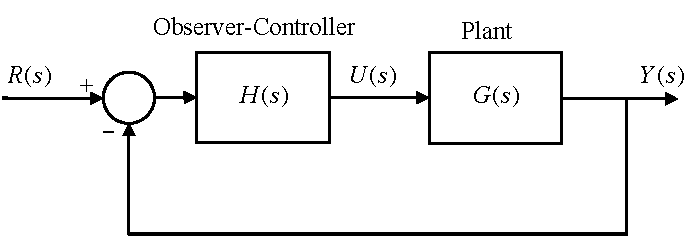
\includegraphics{pictures/fig4.pdf}}
\end{center}
\end{slide}
\fi

\begin{tabular}{|c|c|c|}
\hline
\textbf{Order/Type} & \textbf{ITAE} & \textbf{Bessel}\\
\hline
1 & $s+1$ & $s+1$\\
\hline
2 & $s^2+\sqrt{2}s+1$ & $s^2+\sqrt{3}s+1$\\
\hline
3 & $s^3+1.75s^2+2.15s+1$ & $s^3+2.43s^2+2.47s+1$\\
\hline
etc & etc & etc\\
\hline
\end{tabular}

The above are normalised to give $\omega_0=1$ rad/s. To obtain polynomials for $\omega_0\ne 1$, replace $s$ in the above with $s/\omega_0$.

E.g. if $\omega_0=5$, the $2^\mathrm{nd}$ order ITAE polynomial is: $s^5+5\sqrt{2}s+25$.

\endinput

%%% Local Variables: 
%%% mode: latex
%%% TeX-master: "notes"
%%% End:
\ifslidesonly
\begin{slide}
	\heading{Observer Driven by the Tracking Error (1)}
   \begin{tabular}{|c|c|c|}
\hline
\textbf{Order/Type} & \textbf{ITAE} & \textbf{Bessel}\\
\hline
1 & $s+1$ & $s+1$\\
\hline
2 & $s^2+\sqrt{2}s+1$ & $s^2+\sqrt{3}s+1$\\
\hline
3 & $s^3+1.75s^2+2.15s+1$ & $s^3+2.43s^2+2.47s+1$\\
\hline
etc & etc & etc\\
\hline
\end{tabular}

The above are normalised to give $\omega_0=1$ rad/s. To obtain polynomials for $\omega_0\ne 1$, replace $s$ in the above with $s/\omega_0$.

E.g. if $\omega_0=5$, the $2^\mathrm{nd}$ order ITAE polynomial is: $s^5+5\sqrt{2}s+25$.

\endinput

%%% Local Variables: 
%%% mode: latex
%%% TeX-master: "notes"
%%% End:
\end{slide}
\fi

Now $U=-\mathbf{K}\hat{\mathbf{X}}$, therefore
\begin{eqnarray*}
	U & = &  - \bf{KM}^{ - 1} {\bf{B}}U - {\bf{KM}}^{ - 1} {\bf{L}}\tilde E \\
	U & = &  - \frac{{{\bf{KM}}^{ - 1} {\bf{L}}}}{{1 + {\bf{KM}}^{ - 1} {\bf{B}}}}\tilde E \\
	H\left( s \right) & = &  - \frac{U}{{\tilde E}} = \frac{{{\bf{KM}}^{ - 1} {\bf{L}}}}{{1 + {\bf{KM}}^{ - 1} {\bf{B}}}}
\end{eqnarray*}


\endinput

%%% Local Variables: 
%%% mode: latex
%%% TeX-master: "notes"
%%% End:
\ifslidesonly
\begin{slide}
	\heading{Observer Driven by the Tracking Error (2)}
   Now $U=-\mathbf{K}\hat{\mathbf{X}}$, therefore
\begin{eqnarray*}
	U & = &  - \bf{KM}^{ - 1} {\bf{B}}U - {\bf{KM}}^{ - 1} {\bf{L}}\tilde E \\
	U & = &  - \frac{{{\bf{KM}}^{ - 1} {\bf{L}}}}{{1 + {\bf{KM}}^{ - 1} {\bf{B}}}}\tilde E \\
	H\left( s \right) & = &  - \frac{U}{{\tilde E}} = \frac{{{\bf{KM}}^{ - 1} {\bf{L}}}}{{1 + {\bf{KM}}^{ - 1} {\bf{B}}}}
\end{eqnarray*}


\endinput

%%% Local Variables: 
%%% mode: latex
%%% TeX-master: "notes"
%%% End:
\end{slide}
\fi

A most effective technique is to use optimal control to achieve a compromise between control effort, $u$, and error, $e$.
i.e. Find the feedback vector $\mathbf{K}$ such as to minimise,
\[
J=\int_0^{\infty}\left(e^2+\frac{u^2}{k}\right) dt
\]
where the choice of the parameter $k$ determines the required compromise between,
\begin{itemize}
	\item High Accuracy for High Control Effort (use a large value for $k$)
	\item Lower Accuracy for Reduced Control Effort (use a smaller value for $k$)
\end{itemize}

\endinput

%%% Local Variables: 
%%% mode: latex
%%% TeX-master: "notes"
%%% End:
\ifslidesonly
\begin{slide}
	\heading{Observer Driven by the Tracking Error: $H(s)$}
   A most effective technique is to use optimal control to achieve a compromise between control effort, $u$, and error, $e$.
i.e. Find the feedback vector $\mathbf{K}$ such as to minimise,
\[
J=\int_0^{\infty}\left(e^2+\frac{u^2}{k}\right) dt
\]
where the choice of the parameter $k$ determines the required compromise between,
\begin{itemize}
	\item High Accuracy for High Control Effort (use a large value for $k$)
	\item Lower Accuracy for Reduced Control Effort (use a smaller value for $k$)
\end{itemize}

\endinput

%%% Local Variables: 
%%% mode: latex
%%% TeX-master: "notes"
%%% End:
\end{slide}
\fi

The overall TF is:

\begin{eqnarray*}
	\frac{Y(s)}{R(s)} &=& \frac{G(s)}{1+G(s)H(s)}= \frac{\frac{\alpha_z(s)}{\alpha_p(s)}\times\frac{\alpha_2(s)}{\alpha_1(s)}}{1+\frac{\alpha_z(s)}{\alpha_p(s)}\times\frac{\alpha_2(s)}{\alpha_1(s)}} \\
	\frac{Y(s)}{R(s)} &=& \frac{\alpha_z(s)\alpha_2(s)}{\alpha_p(s)\alpha_1(s)+\alpha_z(s)\alpha_2(s)}=\frac{\alpha_z\alpha_2}{\alpha_c\alpha_e}
\end{eqnarray*}
 



\endinput

%%% Local Variables: 
%%% mode: latex
%%% TeX-master: "notes"
%%% End:
\ifslidesonly
\begin{slide}
	\heading{Observer Driven by the Tracking Error: Overall TF}
   
\begin{eqnarray*}
	\frac{Y(s)}{R(s)} &=& \frac{G(s)}{1+G(s)H(s)}= \frac{\frac{\alpha_z(s)}{\alpha_p(s)}\times\frac{\alpha_2(s)}{\alpha_1(s)}}{1+\frac{\alpha_z(s)}{\alpha_p(s)}\times\frac{\alpha_2(s)}{\alpha_1(s)}} \\
	\frac{Y(s)}{R(s)} &=& \frac{\alpha_z(s)\alpha_2(s)}{\alpha_p(s)\alpha_1(s)+\alpha_z(s)\alpha_2(s)}=\frac{\alpha_z\alpha_2}{\alpha_c\alpha_e}
\end{eqnarray*}
 



\endinput

%%% Local Variables: 
%%% mode: latex
%%% TeX-master: "notes"
%%% End:
\end{slide}
\fi

\begin{itemize}
	\item In this case we see that the overall TF contains the poles of the observer as well as the controller.
	\item Whereas in the normal position changes in the reference input do not excite the error dynamics of the observer, in this configuration they do.
	\item As a result the difference between the observer and the plant states is affected during operation and take further time to settle down.
\end{itemize}

\endinput

%%% Local Variables: 
%%% mode: latex
%%% TeX-master: "notes"
%%% End:
\ifslidesonly
\begin{slide}
	\heading{Observer Driven by the Tracking Error: Comments}
   \begin{itemize}
	\item In this case we see that the overall TF contains the poles of the observer as well as the controller.
	\item Whereas in the normal position changes in the reference input do not excite the error dynamics of the observer, in this configuration they do.
	\item As a result the difference between the observer and the plant states is affected during operation and take further time to settle down.
\end{itemize}

\endinput

%%% Local Variables: 
%%% mode: latex
%%% TeX-master: "notes"
%%% End:
\end{slide}
\fi


% subsection 2_observer_driven_by_the_tracking_error_ (end)

\ifslidesonly
\begin{slide}
	\heading{Summary of this Lecture}
   \begin{itemize}
   	\item Dynamics of the combined controller-observer system
\begin{itemize}
	\item Separation principle
	\item Equivalent classical controller
\end{itemize}
\item Introducing the reference input
\begin{enumerate}
	\item The normal position
	\item Observer driven by the tracking error
\end{enumerate}
   \end{itemize}
\end{slide}
\fi


% section introducing_the_reference_input (end)




%----------------------------------------------------------------
% The end of notes
% ----------------------------------------------------------------
\endinput

%%% Local Variables: 
%%% mode: latex
%%% TeX-master: t
%%% End: 
